\documentclass{minimal}
\usepackage{tikz}
%% \usepackage{pgfmath}

\begin{document}

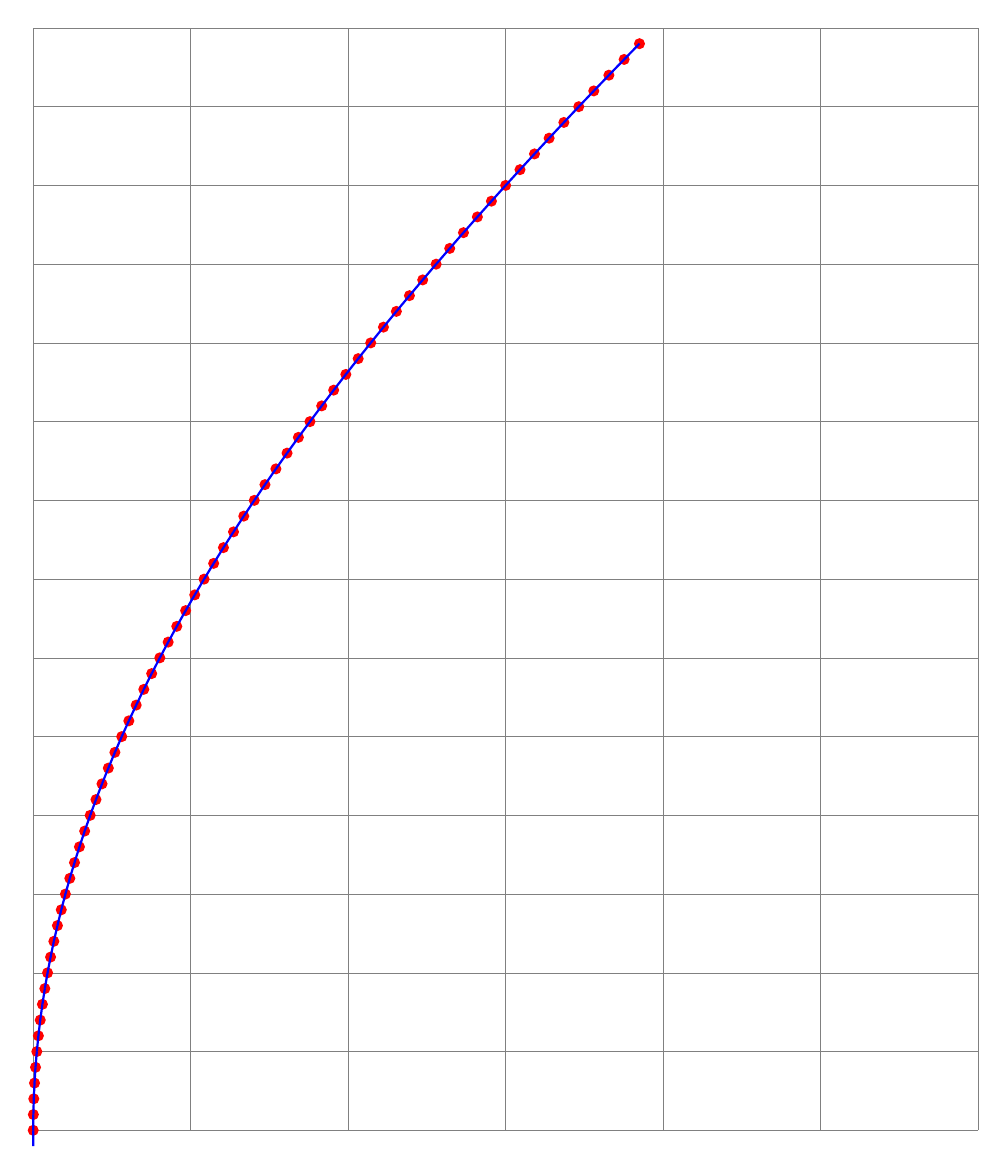
\begin{tikzpicture}[domain=0:60, scale=0.2]
  \draw[very thin,color=gray,xstep=10,ystep=5] (60,0) grid (0,70);
  %% \draw[color=blue] plot (\x,{(sin(90-\x)*70)});
  \foreach \y in {0,...,69} {
    %% \draw[color=green] ({sin(90-\y)},\y) -- ({sin(89-\y),\y});
    %% \fill[red] (\y,\y) circle [radius=16pt];
    %% \draw ({sin(90-\y)},\y) circle [radius=8pt, draw=green, fill=green];
    \fill[red] ({sin(90-\y)*-60+60},\y) circle [radius=10pt];
    \draw[blue, thick] ({sin(90-\y)*-60+60},\y) -- ({sin(90-\y+1)*-60+60},\y-1);
  }
  %% \draw[color=red] plot (\x,{\pgfmathasin(\x)}) node {};
  %% \draw[->] (-0.2,0) -- (4.2,0) node[right] {$x$};
  %% \draw[->] (0,-1.2) -- (0,4.2) node[above] {$f(x)$};
  %% \draw[color=red] plot (\x,\x) node[right] {$f(x) =x$};
  %% % \x r means to convert '\x' from degrees to _r_adians:
  %% \draw[color=blue] plot (\x,{sin(\x r)}) node[right] {$f(x) = \sin x$};
  %% \draw[color=orange] plot (\x,{0.05*exp(\x)}) node[right] {$f(x) = \frac{1}{20} \mathrm e^x$};
\end{tikzpicture}

\end{document}
